\documentclass{article}
\usepackage[utf8]{inputenc}
\parskip = 0.75em
\parindent = 10mm
\def\baselinestretch{1}
\usepackage {float}
\usepackage{listings}
\usepackage{subcaption}
\usepackage[usenames]{color}
\usepackage[numbers,sort&compress]{natbib}
\usepackage{multirow, array}
\usepackage[spanish]{babel}
	\deactivatetilden
	\spanishdecimal{.}
	\addto\captionsspanish{\def\tablename{Tabla}}
	\addto\captionsspanish{\def\listtablename{\'Indice de tablas}}

\usepackage{amsmath,amsfonts,amssymb}
	\allowdisplaybreaks[4]
\usepackage{graphicx}
	\graphicspath{{Figuras/}}
\usepackage[clearempty,pagestyles]{titlesec}
\usepackage{anysize}

\def\baselinestretch{1.5}
\papersize{27.9cm}{21.5cm} 
\marginsize{2cm}{2cm}{1cm}{1cm}

\begin{document}


	\begin{center}
	\huge{\textbf{Tarea 6 Sistema multiagente}}\\
	
	\textsc{ \Large Susana Ruiz Nuñez}
	\end{center}


\section{Planteamiento del problema} 
Se tiene un sistema multiagente \cite{satu} donde hay un conjunto de entidades con estados internos que observan el estado de los otros y reaccionan cambiando su propio estado y su vecindad. Para esta tarea se va a simular un sistema multiagente con aplicación en epidemiología, concretamente el modelo $SIR$: donde los agentes podrán estar en tres estados sucesivamente: susceptibles, infectados, recuperados. Se pide insertar una vacuna al momento de crear los agentes, tales que estos pasen al estado de recuperados sin pasar por la infección.  

\section{Metodología}
Se parte de un código base \cite{satu}, donde ya se tienen representados los principales componentes de la pandemia y su propagación. A partir de este se crea una relación para que aparezcan sujetos recuperados(vacunados) desde el instante incicial. Con la ayuda del lenguaje R se crea un valor probabilidades de vacunar $pv$ que se sustituye por la probabilidad de infección $pi$ en un primer momento, esto garantiza la aparición ude los sujetos vacunados. En un segundo momento con la ayuda de las condicionales se hace que los sujetos susceptibles corran el riesgo de infectarse.




\section{Resultados}
De los resultados obtenidos se puede comentar que a partir de la probabilidad 0.8 de vacunar, el experimento dejó de mostrar datos relevantes por lo que para estas iteraciones no se muestra información. Como se observa en la figura 1, se alcanza el máximo porcentaje de infectados para las probabilidades de vacunación más bajas y mientras se va aumentando dicha probabilidad, es decir, el número de vacunados que se crea al inicio, el pico de infectados disminuye considerablemente.  

\begin{figure}[H]
	\centering
	
	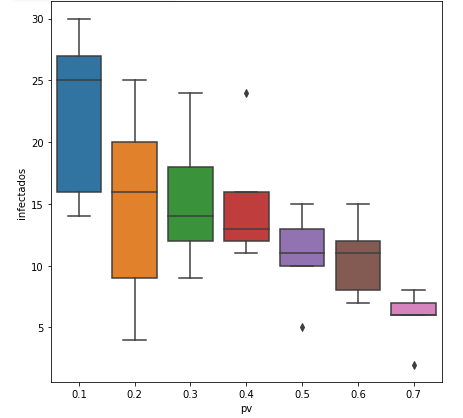
\includegraphics[scale=0.6]{MaxInf.png}
	\caption{Porcentaje de infectados por probabilidad de vacunar}
	\label{fig:f1}
\end{figure}

A continuación se escoge una muestra de datos donde se tienen los valores para algunas probabilidades de vacunación, del porcentaje máximo que alcanzan los infectados y la iteración a la que llega el pico. Como se puede apreciar para las últimas probabilidades se comporta de manera distinta que para las primeras, ya que el pico vuelve a repetirse. En la figura 2 se observa para las cien iteraciones como se comportó el porcentaje máximo de infectados.
\begin{table}[H]
\centering
\caption{Tabla de máximos infectados e iteración donde ocurre }

\begin{tabular}{|c|c|c|}
	\hline
	Probabilidad de vacunación & Máximo infectados & Iteración \\
	\hline
		0.1 & 0.30 & 30 \\
	\hline
	0.3 & 0.24 & 41 \\
	\hline
	0.5 & 0.15 & 59 \\
	\hline
	0.7 & 0.08 & 22 \\
	\hline
	0.8 & 0.04 & 10, 40, 80 \\
	\hline
\end{tabular}
\end{table}



\begin{figure}[H]
	\centering
	\begin{subfigure}[b]{0.45\linewidth}
		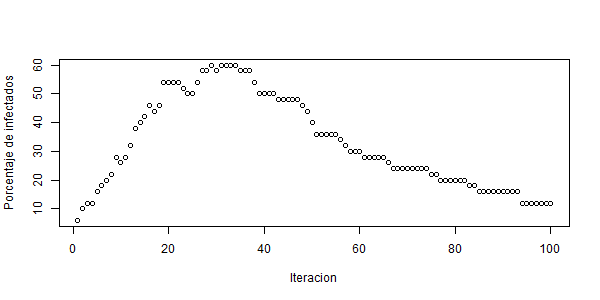
\includegraphics[width=\linewidth]{p6e01.png}
		\caption{Porcentaje de máximos infectados para probabilidad 0.1.}
		\label{1}
	\end{subfigure}
		\begin{subfigure}[b]{0.45\linewidth}
		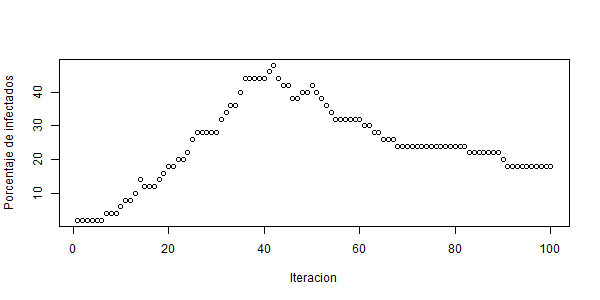
\includegraphics[width=\linewidth]{p6e03.png}
		\caption{Porcentaje de máximos infectados para probabilidad 0.3.}
		\label{2}
	\end{subfigure}
		\begin{subfigure}[b]{0.45\linewidth}
			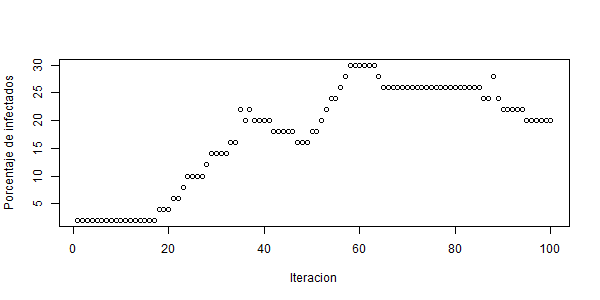
\includegraphics[width=\linewidth]{p6e05.png}
			\caption{Porcentaje de máximos infectados para probabilidad 0.5.}
			\label{3}
	\end{subfigure}
		\begin{subfigure}[b]{0.45\linewidth}
				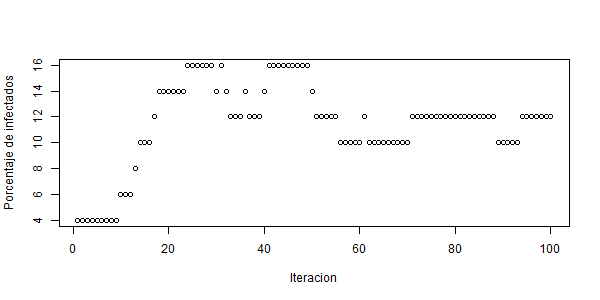
\includegraphics[width=\linewidth]{p6e07.png}
				\caption{Porcentaje de máximos infectados para probabilidad 0.7.}
				\label{4}
	\end{subfigure}
	\caption{Porcentaje de infectados por iteraciones}  		
\end{figure}



\section{Conclusiones}
Se concluye con los experimentos realizados que el porcentaje máximo de infectados disminuye cómo es lógico con el aumento de la probabilidad de vacunar. Mientras más vacunados haya desde un inicio en una pandemia, disminuye la propagación. 

\bibliography{Tarea6}
\bibliographystyle{plainnat}
\end{document} 
